\section{Methodology and Related Work}

\subsection{MoleculeNet}
MoleculeNet~\cite{2018moleculenet} was introduced as a comprehensive benchmark for comparing ML models in molecular sciences, containing a multitude of tasks for molecular property prediction, among others including solubility, toxicity and bioactivity. Previously, there didn't exist a standardized evaluation platform for researchers to compare new machine learning algorithms and datasets were often small, as gathering molecular properties is an expensive task. MoleculeNet therefore aims to create a collection of datasets and evaluation tasks, enabling research teams to create meaningful and easily comparable performance measures for proposed ideas and algorithms. Furthermore MoleculeNet comes with a suite of tools to create and adapt ML models, containing implementation of many existing featurizers and algorithms for molecular machine learning. While we used the datasets from MoleculeNet, we accessed them through the Open Graph Benchmark python package.

\subsection{Open Graph Benchmark}
Open Graph Benchmark (OGB)~\cite{2021ogb} is a framework for benchmarking machine learning on graphs, providing large-scale, real world datasets as well as an easy to use software framework for loading  datasets and evaluating model performance.
For comparing model performances, OGB provides leaderboards for different datasets and challenges, split into the sections Node Property Prediction, Link Property Prediction and Graph Property Prediction, as well as a large-scale challenge~\cite{hu2021ogblsc} leaderboard, which aids comparison of performance on very large graphs.

Our main focus will be Graph Property Prediction, mainly on the datasets provided by MoleculeNet, those can be seen in~\autoref{table:ogb_mol_datasets}. All datasets are derived from MoleculeNet and added to OGB, each one respectively providing a large amount of molecules for molecular property prediction for different task types. Molecules are represented by graphs, where atoms are the nodes and corresponding chemical bonds are represented by the edges. Node features are represented as a 9-dimensional vector, edge feature vectors are 3-dimensional, the respective value ranges can be seen in \autoref{table:node_feature_list} and \autoref{table:edge_feature_list}.

\begin{table}[h!]
    \centering
    \begin{tabular}{@{}lrrlr@{}}
        \toprule
        name             & graphs & tasks & task type             & max fraction positive \\ \midrule
        ogbg-molhiv      & 41127  & 1     & binary classification & 0.035086              \\
        ogbg-molpcba     & 437929 & 128   & binary classification & 0.143402              \\
        ogbg-moltox21    & 7831   & 12    & binary classification & 0.120291              \\
        ogbg-molbace     & 1513   & 1     & binary classification & 0.456709              \\
        ogbg-molbbbp     & 2039   & 1     & binary classification & 0.765081              \\
        ogbg-molclintox  & 1477   & 2     & binary classification & 0.936357              \\
        ogbg-molmuv      & 93087  & 17    & binary classification & 0.000322              \\
        ogbg-molsider    & 1427   & 27    & binary classification & 0.923616              \\
        ogbg-moltoxcast  & 8576   & 617   & binary classification & 0.205340              \\
        ogbg-molesol     & 1128   & 1     & regression            & na                    \\
        ogbg-molfreesolv & 642    & 1     & regression            & na                    \\
        ogbg-mollipo     & 4200   & 1     & regression            & na                    \\ \bottomrule
    \end{tabular}
    \caption{the molecule datasets from ogb}
    \label{table:ogb_mol_datasets}
\end{table}

\begin{table}[!ht]
    \parbox{.49\linewidth}{
        \centering
        \begin{tabular}{lll} % TODO  Value Range should be replaced by data type
            \toprule
            index & feature            & feature type \\ \midrule
            0     & atom number        & multi-class  \\
            1     & chirality          & multi-class  \\
            2     & degree             & multi-class  \\
            3     & formal charge      & multi-class  \\
            4     & number of H-atoms  & multi-class  \\
            5     & number of radicals & multi-class  \\
            6     & hybridization      & multi-class  \\
            7     & is aromatic        & binary-class \\
            8     & is in ring         & binary-class \\ \bottomrule
        \end{tabular}
        \caption{Node feature vector}
        \label{table:node_feature_list}
    }
    \hfill
    \parbox{.49\linewidth}{
        \centering
        \begin{tabular}{lll}
            \toprule
            index & feature       & feature type \\\midrule
            0     & bond type     & multi-class  \\
            1     & bond stereo   & multi-class  \\
            2     & is conjugated & binary-class \\\bottomrule
        \end{tabular}
        \caption{Edge feature vector}
        \label{table:edge_feature_list}
    }
\end{table}

We decided to use OGB as a benchmarking framework instead of the MoleculeNet benchmark results, because OGB submissions are much more versatile and active, containing results from many research teams with the latest submission for ogb-molhiv dating to May 2022, contrary to the MoleculeNet results which were provided by the authors of the paper only and are dated to January 2018.

\subsection{Doc2Vec}
Doc2Vec is a widely used method for obtaining distributed representations of documents as continuous vectors in a low-dimensional space, also known as paragraph embeddings. Doc2Vec, introduced by Le and Mikolov~\cite{2014doc2vec}, was built as an extension of the popular Word2Vec algorithm~\cite{mikolov2013distributed} to the domain of entire documents and together with Word2Vec builds the base for many ideas regarding graph embedding.

Doc2Vec learns a vector representation for each document in a corpus by utilizing so called Paragraph Vectors. The architecture is similar to that of Word2Vec but includes an additional vector representation for each document. There are two ways to obtain document vectors: Distributed Memory version of Paragraph Vector (PV-DM) and Distributed Bag of Words version of Paragraph Vector (PV-DBOW).

In the PV-DM model, the document vector is trained to predict the next word in a randomly sampled sequence of words, with the document vector and a window of surrounding words as input. The document vector is then updated alongside the word vectors during backpropagation. This model captures the overall topic and meaning of the document, as it has access to all words in the document.

On the contrary, the PV-DBOW model doesn't pay attention to the order of words and only utilizes the occurrence information of words in the document. The input to this model is a bag of words from a randomly sampled window with the task to predict the words in the window. The document vector is trained alongside the word vectors, and  aims to represent the document's overall semantic content.

In both models, the document vector is learned by optimizing a loss function, typically the negative log-likelihood of predicting the target words. The resulting document vectors are continuous, dense, and low-dimensional, making them suitable for various downstream tasks, such as document classification, clustering, and information retrieval.

Doc2Vec has been shown to outperform other methods for document embeddings in several benchmark datasets and downstream tasks. This idea of capturing the semantics and meaning of the documents was the basis for many future implementations and also laid the path for good algorithms regarding graph embedding.

\subsection{Graph Embedding}
Graph embedding is a technique in graph machine learning that maps nodes, edges or whole graphs into a low-dimensional vector space while preserving the graph structure and semantic information. This technique has become increasingly popular due to its usefulness in various applications such as social network analysis, recommendation systems and molecular sciences.

The goal for this technique is to produce a vector which can be used as input for various existing machine-learning models and techniques, elevating their usefulness to graphs. To achieve a good representation for those graphs, local and global structural information has to be encoded into such vectors.

Graph Embedding was visualized very nice by Google Research~\cite{epasto2019embedding} as seen in \autoref{fig:graph_embedding}. As seen here, overlapping communities are pulled apart while similar nodes are grouped together.

\begin{figure}[h!]
    \centering
    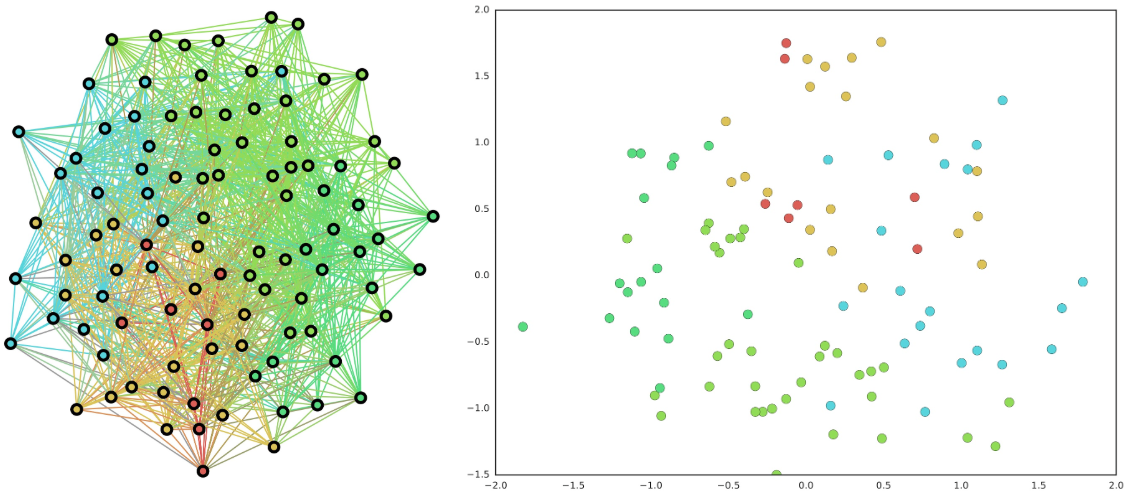
\includegraphics[scale=0.35]{tex/res/graph_embedding.png}
    \caption{Embedding of a graph with overlapping communities using Node2Vec \tiny{source: \cite{epasto2019embedding}}}
    \label{fig:graph_embedding}
\end{figure}

There is a multitude of different ideas and methods to create graph embeddings, we will focus mainly on random walk embeddings and deep learning approaches, to be exact most methods are combinations of those ideas~\cite{2017graph2vec,2016node2vec,2021graphormer}.
\subsubsection{Node2Vec}

Node2Vec, presented by Grover and Leskovec in 2016~\cite{2016node2vec}, is a framework for learning low-dimensional representations of nodes in large-scale networks. The goal of Node2Vec is to learn embeddings that capture the structural information of nodes, such as their connectivity patterns, in a way that is useful for downstream tasks, such as node classification, clustering, and link prediction, i.e. lowering the complexity of large network structures and encapsulating as much information as possible in a less complex structure, as seen in~\autoref{fig:graph_embedding}.

Node2Vec builds on the skip-gram model, which is popular in NLP problems and works by learning word embeddings through predicting the context of a given word. Correspondingly, Node2Vec learns node embeddings by training a neural network to predict the context of a given node, where the context of a node is defined as the set of nodes that are likely to appear in random walks starting from that node.

Node2Vec uses a biased random walk strategy, that balances the trade-off between exploring the whole, large network and staying in the local neighborhood of a node. Each walk starts at a given node choosing for each step to either revisit the previous node or move to the next one based on two parameters: the in-out degree bias  $p$ and the return bias $q$, where $p$ controls the likelihood of staying in the same community, while $q$ controls the likelihood of visiting a node that is further away from the current one. Node2Vec can generate different types of random walks by changing these parameters, which are able to capture different types of structural information of the network.

After the random walks are generated, Node2Vec uses the skip-gram model to learn node embeddings by maximizing the likelihood of predicting the correct context nodes given the current node. To train the skip-gram model, negative sampling is used, which samples negative nodes that are not in the context set and adjusts the embedding vectors to minimize the difference between the predicted and actual context sets.

Node2Vec has several advantages over previous methods for network embedding. Although being scalable to large networks and being able to handle diverse networks with multiple types of nodes and edges, it can still capture both the local and global structure of the network by tuning the $p$ and $q$ parameters. Additionally, it can handle noisy or incomplete networks by incorporating information from the context nodes, alleviating missing data.

In conclusion, Node2Vec is a performant and popular node embedding model that can be applied to a wide range of downstream tasks, such as link prediction, node classification, and community detection.

\subsubsection{Graph2Vec}
Graph2Vec is a method for unsupervised learning of distributed representations of graphs proposed by Narayanan et al.~\cite{2017graph2vec}. This approach builds on top of the previously described Doc2Vec method, but contrary to learning representations for words or paragraphs, it learns representations for whole graphs, that can be of arbitrary size.

Graph2Vec works by initially generating a set of subgraphs for each graph in the dataset, which can be seen as 'context graphs'. Those context graphs are then used to train a skip-gram neural network to learn embeddings for all graphs.

Context graphs are generated by performing a random walk on the whole graph. The next node to be selected during each step of the walk is chosen according to its distance to the currently selected one. The resulting sequence of nodes is then used to generate a set of subgraphs which are added to a pool of context graphs.

After that, once again the skip-gram model is used to learn embeddings for the graphs. Each graph is represented as a bag-of-context, i.e., a set of subgraphs that appear in the context of the graph and the skip-gram model then learns to predict the context graphs of a input graph, given the graph's embedding.

The skip-gram model used in Graph2Vec is similar to the one used in Word2Vec, but instead of predicting the neighboring words of a given word, it predicts the context graphs of a given graph. The model takes as input a graph embedding and a context graph, and predicts whether the context graph appears in the bag-of-context-graphs of the input graph.

Graph2Vec uses a negative sampling technique that is similar to the one used in Doc2Vec to train the model whose objective it is to maximize the probability of predicting the correct context graphs of a given graph, while minimizing the probability of predicting randomly sampled negative context graphs.

The resulting embeddings capture the structural properties of the graphs, allowing them to be used for various downstream tasks. In our case, we will mainly use Graph2Vec as a benchmark and reference point.

All discussed "2Vec" models are methods for unsupervised learning, meaning they don't need labeled input data. This is a key advantage in the usage of those methods, as they can easily be used for many different applications while not depending on existing labeled data, additionally, large amounts of data can be used to improve model performance.

\subsection{Transformers}
In 2017 Vaswani et al. proposed a new network architecture for Natural language processing (NLP) problems, called the Transformer~\cite{vaswani2017attention}. Abstractly speaking, Transformers consider input sentences as a connected system of words, thus attending on all other words while learning the meaning of one specifically.

The Transformer architecture is build of many layers, each containing a self-attention module and a position-wise feed-forward network. Self-attention is then calculated as described in~\cite{2021graphormer}:

\begin{align}
    Q = HW_Q,\quad K = HW_K,\quad V = HW_V,\label{eqn:attention-alpha} \\
    A = \frac{QK^\top}{\sqrt{d_K}}, \quad \attn{H} = \softmax{A}V,     \\
    FFN(x) = \max(0,xW_1 + b_1)W_2 + b_2
    \label{eqn:attention-alpha2}
\end{align}

Here $Q$, $K$, and $V$ are calculated by multiplying the input $H$ of the attention module with the respective matrices $W_Q\in\Rbb^{d\times d_K}, W_K\in\Rbb^{d\times d_K}$ and $ W_V\in\Rbb^{d\times d_V}$ which then represent Queries, Keys and Values of the attention module. Those matrices are learnable and are produced during the training of the model.

Queries are basically one-hot feature vectors, representing the features of interest, which are then multiplied with the transposed Key matrix to get feature specific masks (denoted as $A$ above). Those masks are then used during attention to isolate specific features from the values (denoted in $\attn{H}$ above), increasing the correctness of value predictions.

$d$ denotes the hidden dimensions, which in case of single-head self-attention is the same as $d_K$ and $d_V$. The hidden dimension is the dimension of the key vectors, in case of \cite{vaswani2017attention} this was $64$.This leads to the equation for the attention matrix above and its adaption for Graphormer in \autoref{eqn:attention-matrix}. The result of this equation is the softmax score, which is then multiplied with the Value vectors. The sum of those weighted vectors is the output of the self-attention module. By doing this, other tokens of the input which are seen as relevant, will continue upwards while non relevant tokens are drowned with a small softmax score.

After each self-attention module follows a feedforward neural network, denoted in line $(3)$ of \autoref{eqn:attention-alpha2}. During this step, ReLU is used to drown out negative values, $x$ are masked word activities, $(W_1 + b_1)$ denotes a multi-word feature creation matrix and $(W_2 + b_2)$ is a transition matrix.

As Transformer models achieved astonishing performance for NLP problems, they laid the path for a lot of research. Many teams tried to adapt the idea to graph machine learning, leading to interesting findings and proposals of many performant models, all using Transformer architecture as their starting point. Transformers and adaptions for graphs are used in GraphGPS~\cite{2023graphgps}, which we will describe later and use as a testing framework to compare different approaches to graph embedding.
\subsection{Graph Transformers}
After the success of Transformers for NLP problems~\cite{kalyan2021ammus}, many researchers tried adapting the ideas of Transformer for graph machine learning problems, taking advantage of the benefits of global attention in graph models, thus a multitude of graph transformer models~\cite{dwivedi2021generalizationTransformer,2021graphormer,kreuzer2021rethinking,mialon2021graphit,wu2022representing} were published. Many of those ideas were leveraged in GraphGPS~\cite{2023graphgps}, as described in \autoref{sec:graphgps} and \autoref{sec:graphgps_hig}.

\subsubsection{Graph Transformer Networks}
GTNs, proposed by Dwivedi et al.~\cite{dwivedi2021generalizationTransformer}, are designed to leverage graph sparsity and positional encodings and add them as a bias during self-attention. Attending to the whole graph is often not feasible because of graph size and node count, therefore GTNs only attend to the local neighborhood of nodes. Additionally, positional encodings are leveraged, to alleviate the missing structural information using Transformers, thus encoding important graph structural information into the Transformer. Positional encodings are created using Laplacian eigenvectors~\cite{belkin2003laplacian}, which are added to the node features.

The key differences of GTNs with respect to original Transformers are the following: Neighborhood connectivity is used as the function for the attention mechanism, which is done by computing a weighted sum of the surrounding node embeddings. Positional encodings are replaced by Laplacian eigenvectors, which are precomputed for each graph and additionally, edge representations are added, to engrain important edge information into the model. Those edge features are learned by a separate feed-forward neural network, which takes the concatenated node embeddings as an input and the resulting edge features are again used in self-attention to update node embeddings.


\subsubsection{Graphormer}
As an adaption of Transformers~\cite{vaswani2017attention} for graph representation learning, Graphormer~\cite{2021graphormer} was presented by Ying et al., providing a performant Transformer model, excelling in various graph representation learning tasks, particularly for complex structures.

Graphormer achieves such good results by introducing three types of encodings as a bias to the self-attention mechanism used in Transformer architecture. While Transformer models work by computing weighted sum of input features based on attention scores between different tokens during self-attention, Graphormer incorporates structural information of different nodes in pairwise relation to each other into the self-attention mechanism, thus increasing the information encapsuled in the self-attention module, which is held by graph structures and features present.

To capture information about the importance of a node in a given network, Graphormer uses a measure called node centrality by utilizing degree centrality of a given node. This is done by introducing learnable embedding vectors, one for the degree of ingoing edges and one for the outgoing ones. Those vectors are scalars which are added to the features of each node, so node importance and semantic correlation are respected during self-attention. Those scalars are indexed from two vectors according to the respective degrees as seen in \autoref{fig:graphormer_centr_enc}.

\begin{figure}[h!]
    \centering
    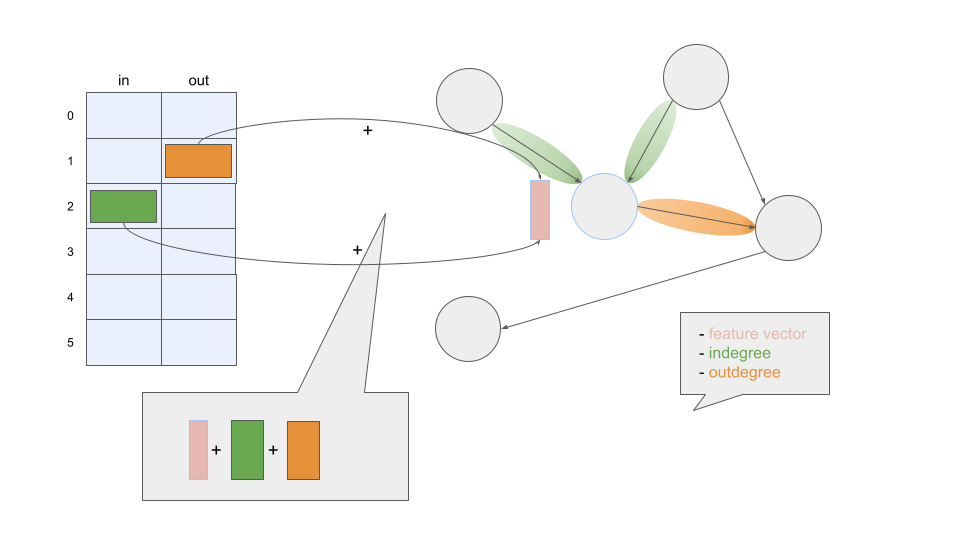
\includegraphics[scale=0.35]{tex/res/graphormer_centr_enc.png}
    \caption{Centrality Encoding: learnable embedding vectors are added to feature vectors of nodes}
    \label{fig:graphormer_centr_enc}
\end{figure}

The other two encodings are added as bias to the Attention Module used in Transformers as described in \autoref{fig:graphormer_att} and the following equation.
\begin{equation}
    A_{ij} = \frac{(h_i W_Q)(h_j W_K)^T}{\sqrt{d}} + b_{\Phi (v_i, v_j)} + c_{ij}
    \label{eqn:attention-matrix}
\end{equation}

\begin{figure}[h!]
    \centering
    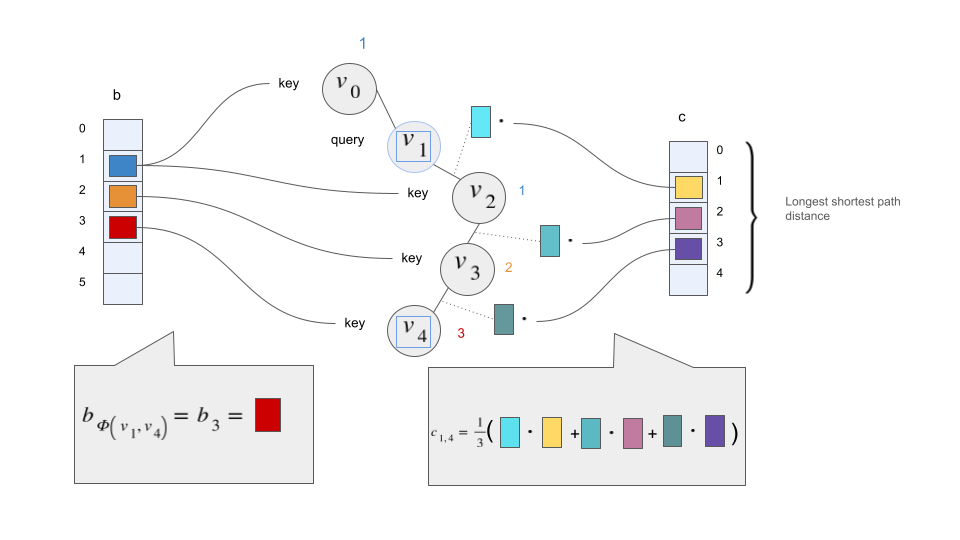
\includegraphics[scale=0.35]{tex/res/graphormer_attention.png}
    \caption{Spatial Encoding (left) and Edge Encoding (right) added as bias to Attention Module}
    \label{fig:graphormer_att}
\end{figure}

The bias $b_{\Phi (v_i, v_j)}$ is produced by the so called spatial encoding, which captures positional information for each node with respect to the network. This is achieved by using the distance of the shortest path between two connected nodes, described by the function $\Phi$, combined with a learnable vector which is indexed according to $\Phi$. The resulting scalar is added as bias in the self-attention module.

By doing that, the model can attend to a more relevant subset of the network according to the task. An example given in the paper is the possibility to increase attention to nodes surrounding a given node instead of nodes which lay further away.

Finally Graphormer introduces a method to include edge information in the model by adding an the additional bias term $c_{ij}$ to the attention module~(\autoref{eqn:bias_2}). This bias is created by averaging the dot-products of edge features ($x_{e_n}$) and a learnable scalar ($(w_n^E)^T$), which is indexed according to the distance of the edge to the start node for each edge along the shortest path between each two connected nodes.

\begin{equation}
    c_{ij} = \frac{1}{N} \sum_{n=1}^{N} x_{e_n}(w_n^E)^T
    \label{eqn:bias_2}
\end{equation}

\subsection{GraphGPS}
\label{sec:graphgps}
L. Rampásek et al. introduced GraphGPS in their paper 'Recipe for a General, Powerful, Scalable Graph Transformer.'~\cite{2023graphgps} The objective of this model recipe is to provide a foundation for incorporating structural and positional information into node and edge features, while maintaining the flexibility of the model that implements these features.

GraphGPS serves as a preprocessor for the actual model learning on the dataset. The authors tested GraphGPS with several models, such as Transformer~\cite{vaswani2017attention}, Performer~\cite{choromanski2022performer}, BigBird~\cite{zaheer2021bigbird}, GatedGCN~\cite{bresson2018GatedGCN}, and more. They designed it to allow models that permit only Node Features, known as the Global Attention layer, as well as models that permit both Node and Edge Features, known as the MPNN layer. Both layers can also be used in combination to integrate the distinct advantages of two models.

The authors categorized structural and positional information into two types since the distance between nodes, although indicating the graph's structure, is insufficient to capture structural similarities. They incorporated this information by utilizing structural and positional encodings (SE and PE), which are divided into Local, Global, and Relative categories. Local and Global encodings are implemented as node features, while Relative encodings are implemented as edge features.

\begin{figure}[h!]
    \centering
    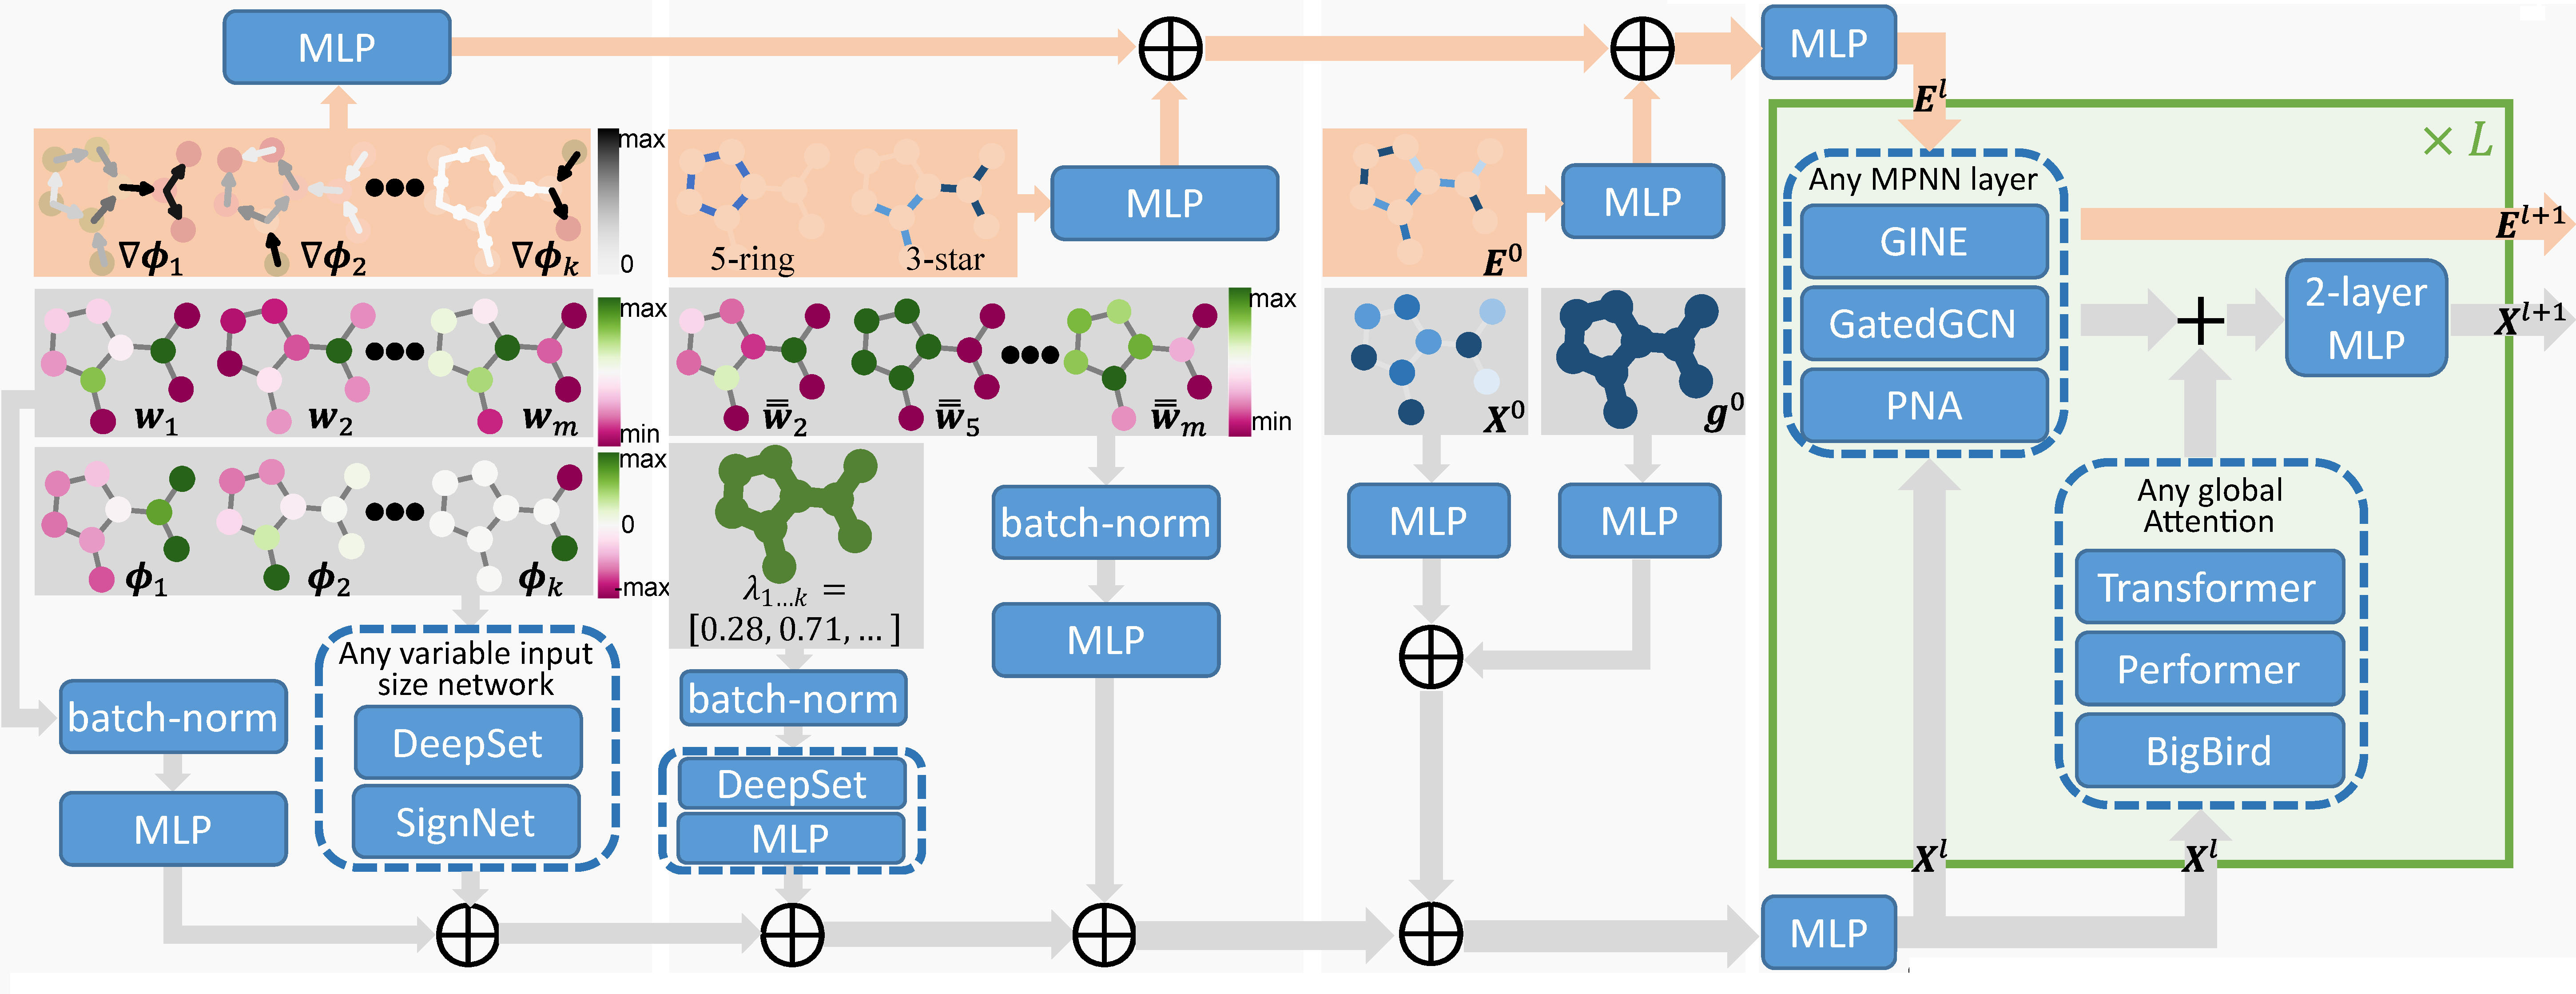
\includegraphics[scale=0.13]{tex/res/gps_abstract.png}
    \caption{General overlook of GraphGPS taken from~\cite{2023graphgps}}
    \label{fig:gps-abstract}
\end{figure}

\subsection{Heterogeneous Interpolation on Graphs}
A winning entry for the dataset ogb-molpcba, called HIG-GraphClassification~\cite{tencenc2021Hig,tencenc2021HigPaper} was submitted to the OGB leaderboard in 2021 by Wang et al., providing an implementation and a brief technical report describing the research. By using their method combined with Graphormer, they were able to achieve better average precision than all previous submissions.

The report introduces heterogeneous interpolation, which is done by dropping the feature vectors of several randomly selected nodes and replacing them by the interpolated feature mix of all neighboring nodes.
By using a mixing ratio, the influence of each neighbors features can be adapted. To account for possible information loss, KL-Divergence constraint loss is added. By doing that, the distributions of two identical graphs remain similar, even after interpolating some feature vectors. The general idea was visualized by Wang et al. in \autoref{fig:hig_figure}.

\begin{figure}[h!]
    \centering
    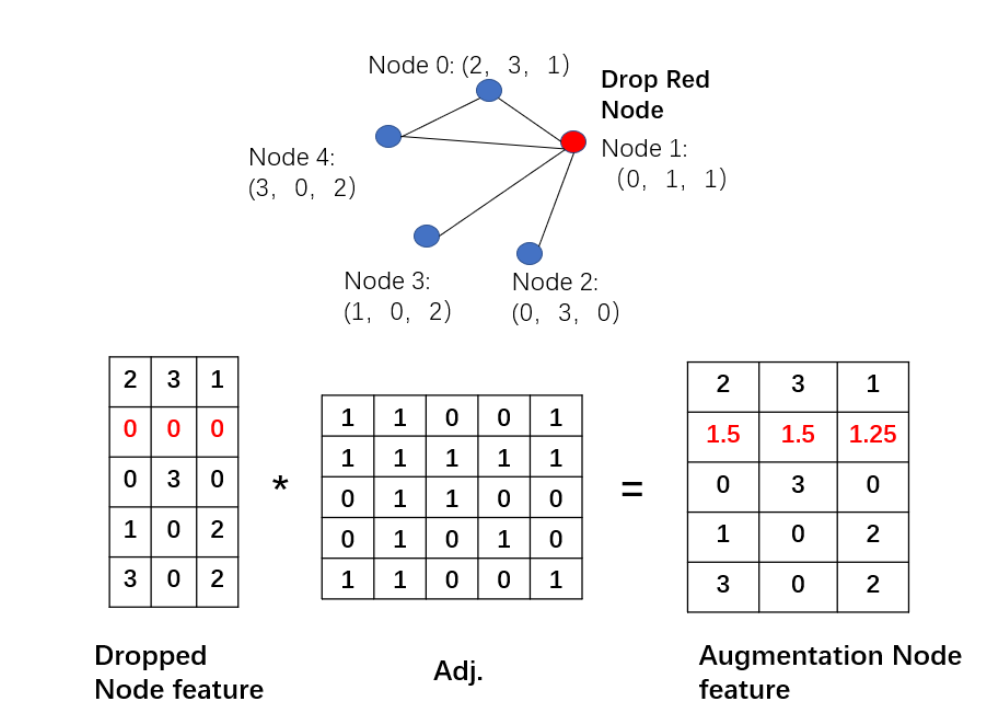
\includegraphics[scale=0.3]{tex/res/hig_figure.png}
    \caption{Visualization of HIG-GraphClassification by Wang et al., taken from \cite{tencenc2021HigPaper}}
    \label{fig:hig_figure}
\end{figure}

We combine the idea of interpolating feature vectors of neighboring nodes with GraphGPS to test performance with different embedding methods.